\appendix

\chapter{Resultados anecdóticos}

\begin{table}[h]
  %% \begin{minipage}[c]{0.7\linewidth}
  %%   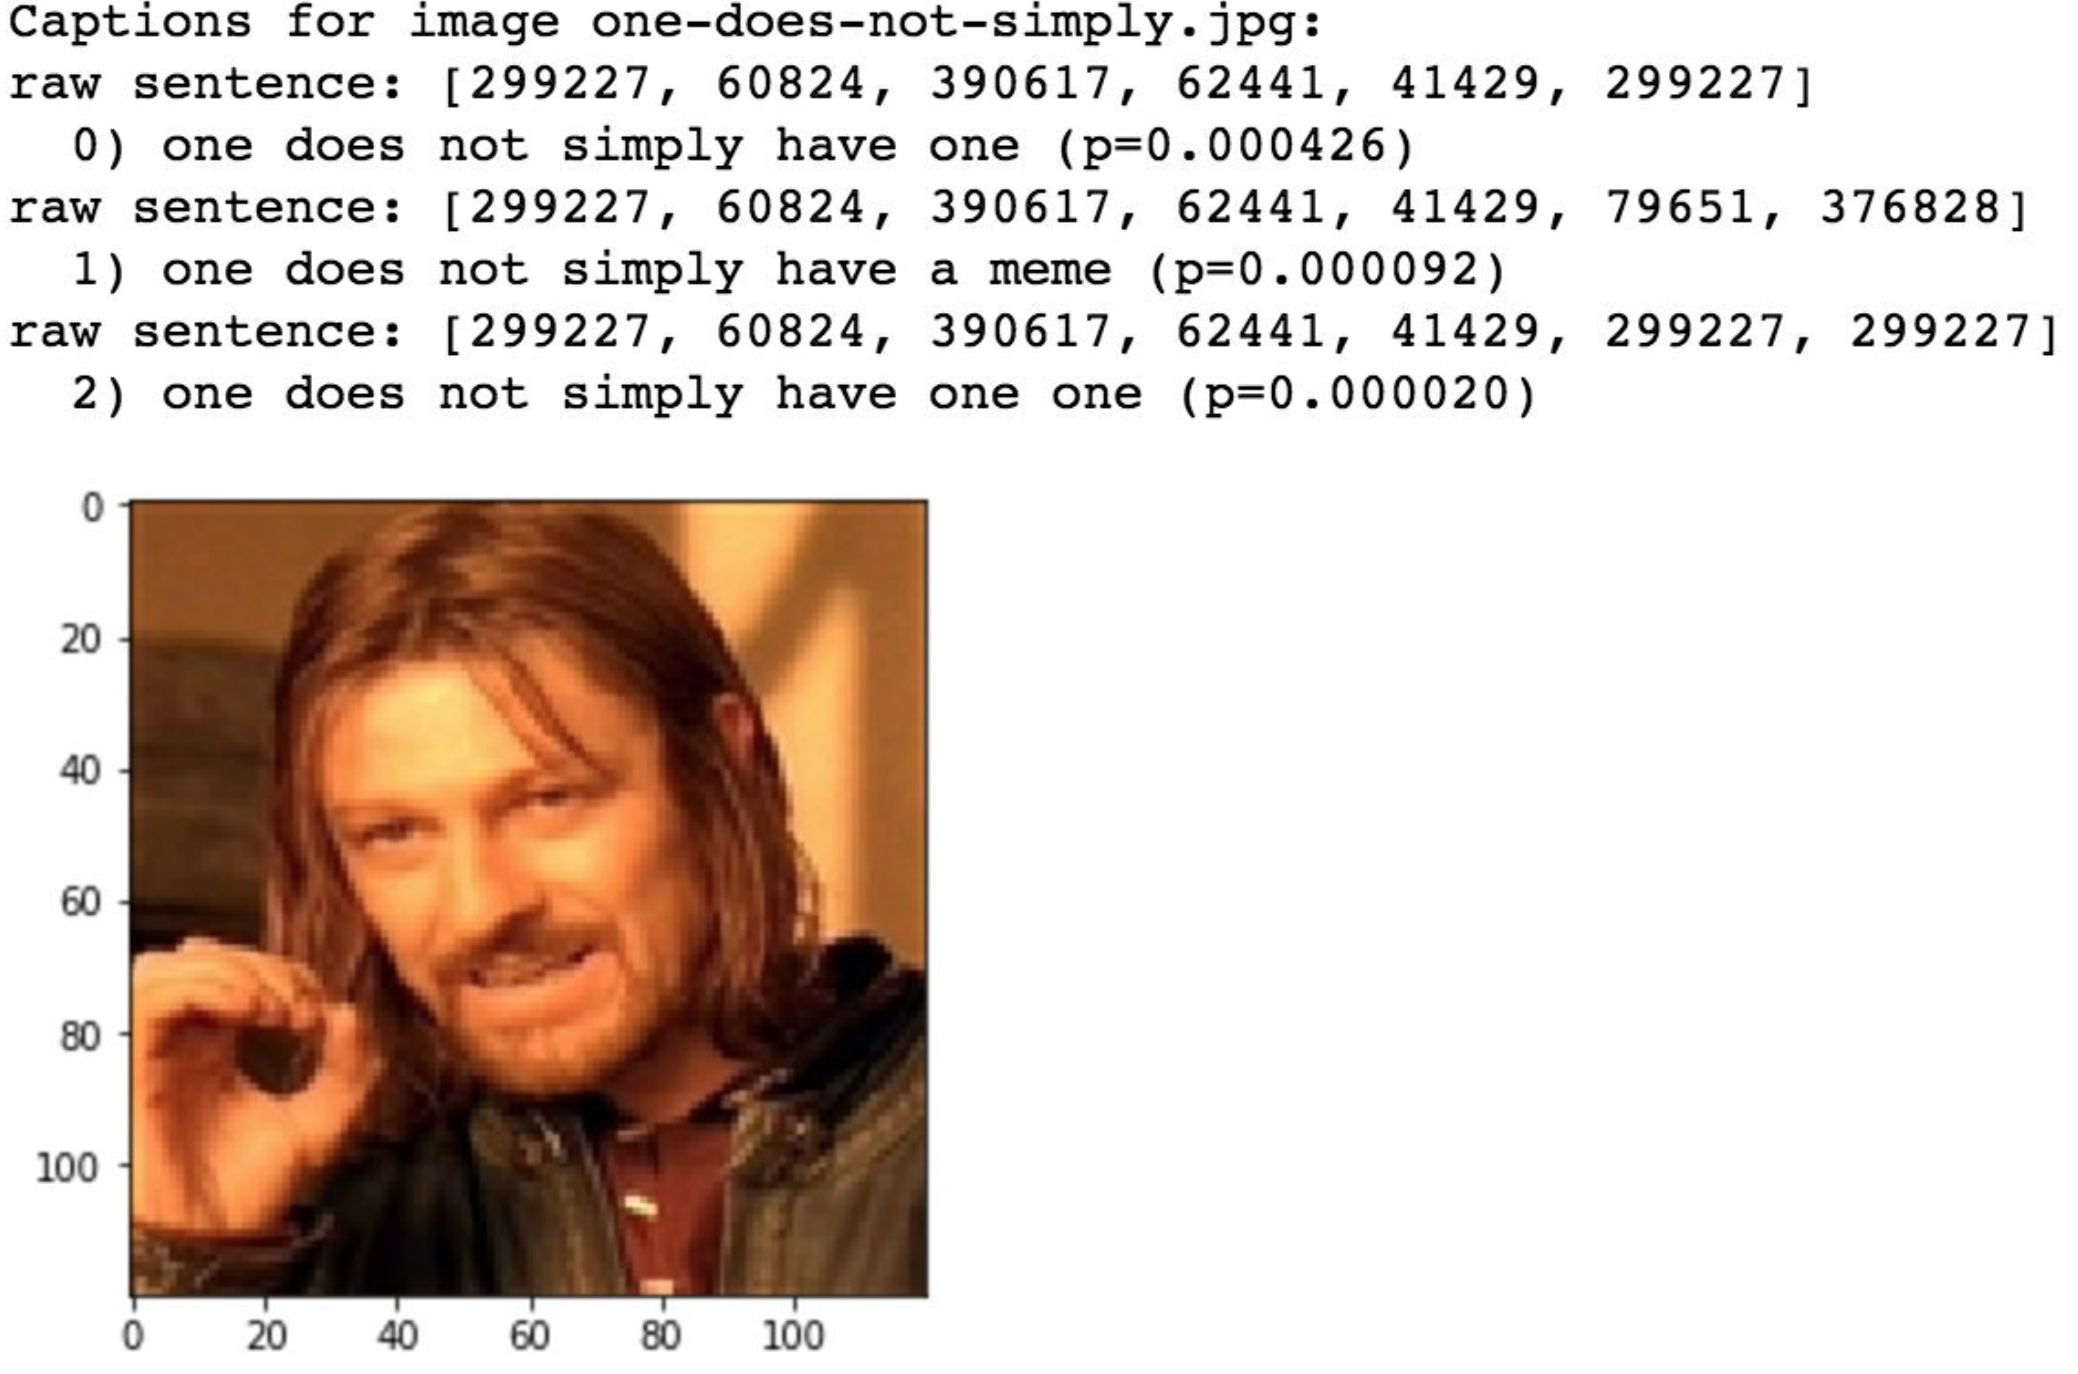
\includegraphics[width=\linewidth]{exp5-anec-1}
  %% \end{minipage}\hfill
  %% \begin{minipage}[c]{0.4\linewidth}
  %%   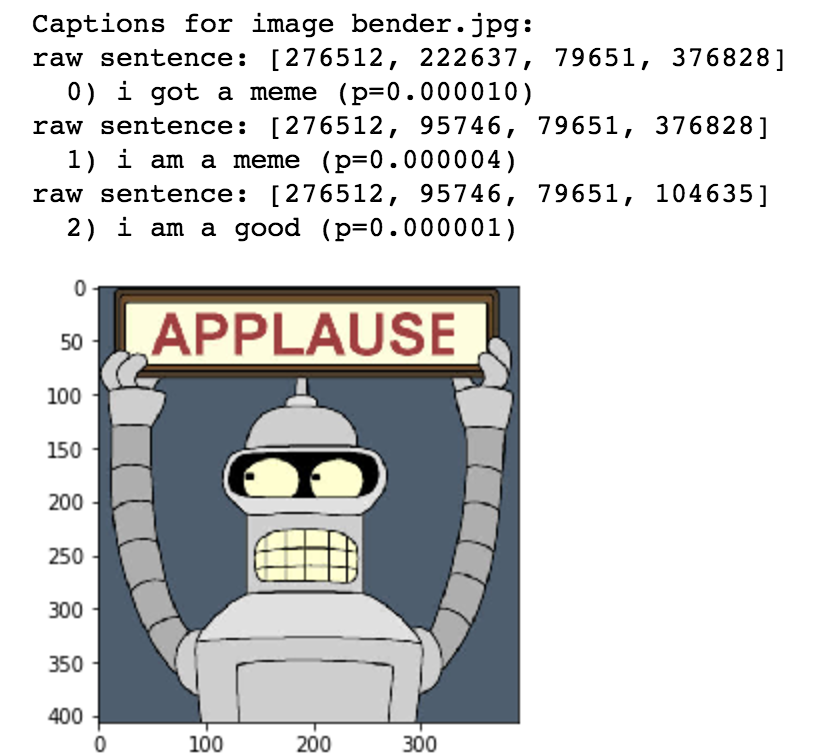
\includegraphics[width=\linewidth]{exp5-anec-2}
  %% \end{minipage}
  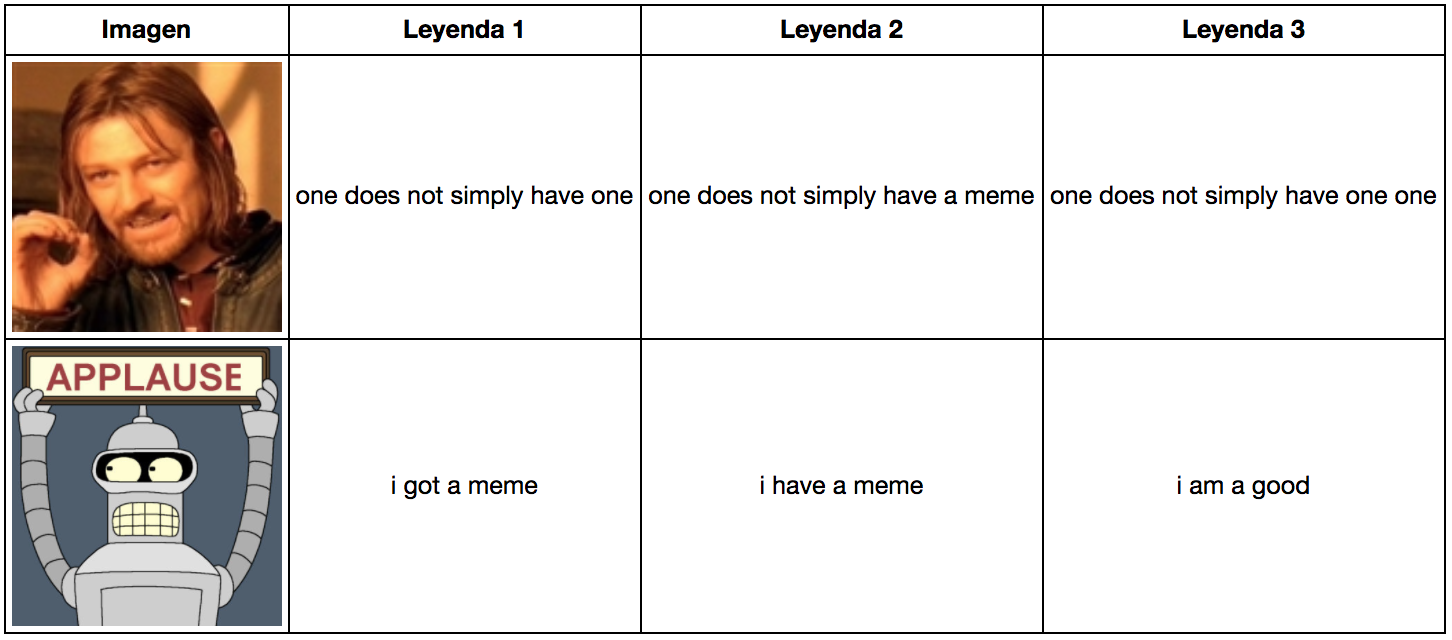
\includegraphics[width=\linewidth]{exp5-anec}
  \caption{
    Resultados \emph{anecdóticos} del entrenamiento de la LSTM, con previa afinación\
    de \emph{Inception V3}. Como el orden en los tensores de entrenamiento está determinado\
    por cada personaje, ocurrió un sobreajuste durante ciertas épocas contiguas. Esto se\
    muestra mediante la repetición de frases muy características en la elaboración de\
    leyendas.
    (Fuente: elaboración propia.)
  }
  \label{exp5:anec}
\end{table}

\begin{table}[h]
  %% \begin{minipage}[c]{\linewidth}
  %%   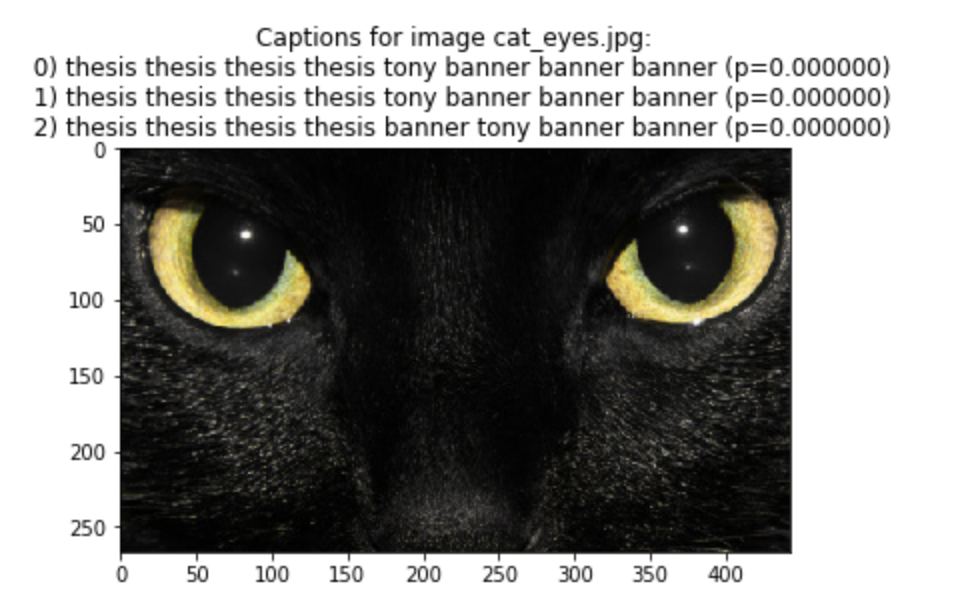
\includegraphics[width=\linewidth]{exp6-anec-1}
  %% \end{minipage}\hfill
  %% \begin{minipage}[c]{\linewidth}
  %%   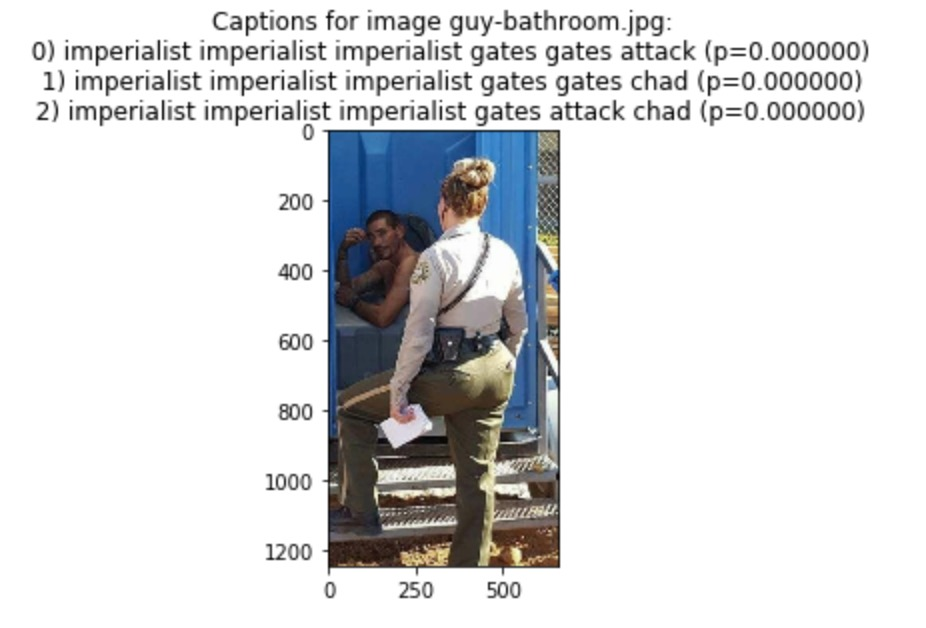
\includegraphics[width=\linewidth]{exp6-anec-2}
  %% \end{minipage}
  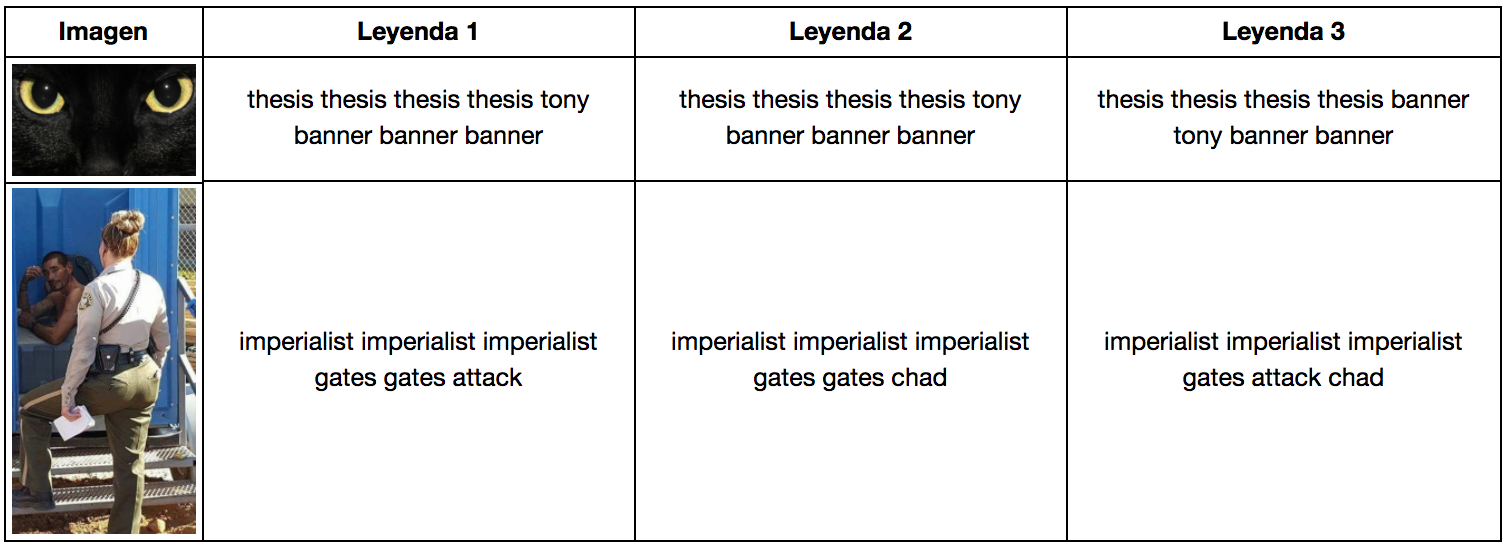
\includegraphics[width=\linewidth]{exp6-anec}
  \caption{
    Resultados \emph{anecdóticos} del entrenamiento de la LSTM, con previa afinación\
    de \emph{Inception V3} y reducción del vocabulario. Se puede apreciar la repetición\
    de palabras, como principal característica.
    (Fuente: elaboración propia.)
  }
  \label{exp6:anec}
\end{table}

\begin{table}[h]
  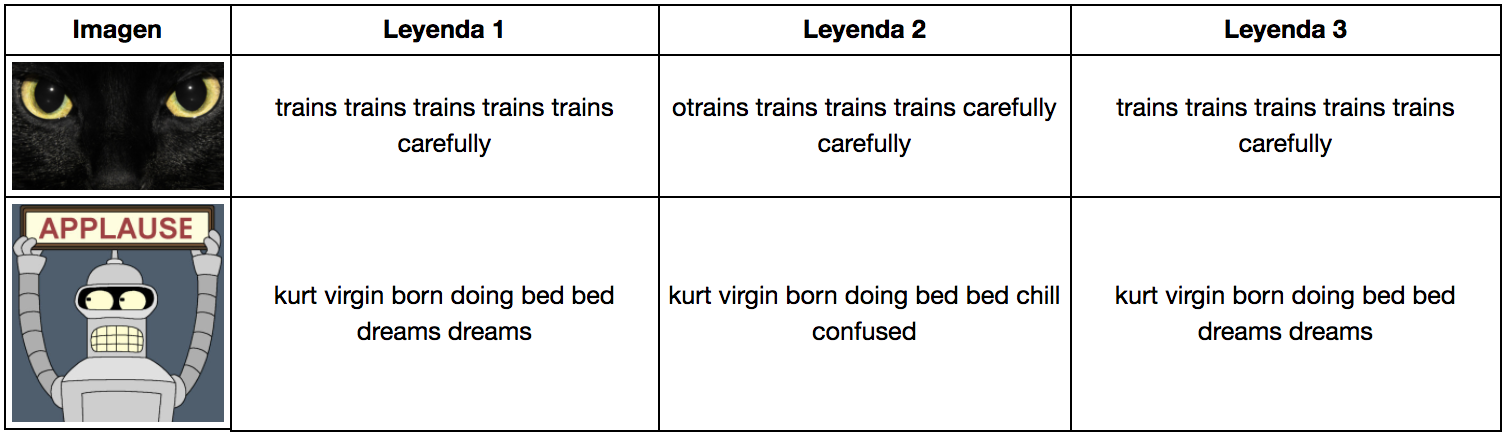
\includegraphics[width=\linewidth]{exp7-anec}
  %% \begin{minipage}[c]{\linewidth}
  %%   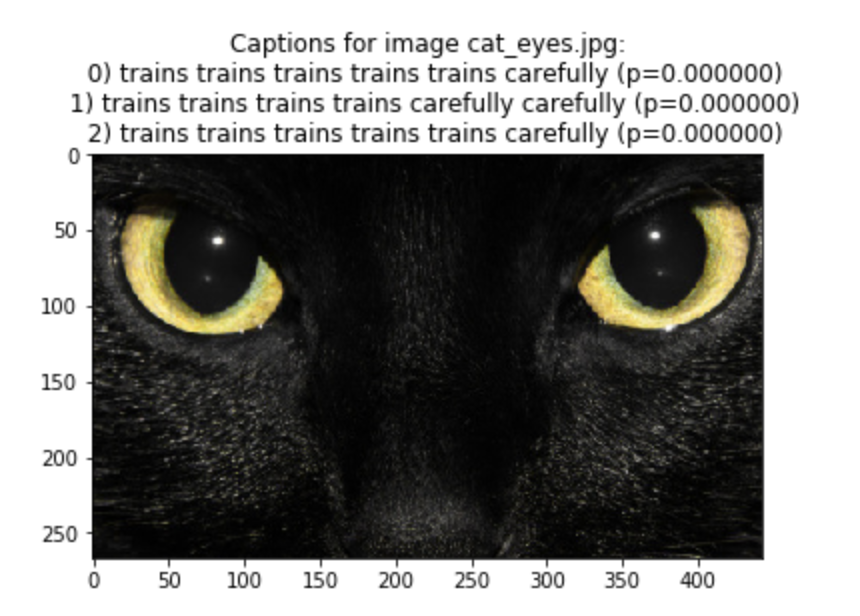
\includegraphics[width=\linewidth]{exp7-anec-1}
  %% \end{minipage}\hfill
  %% \begin{minipage}[c]{\linewidth}
  %%   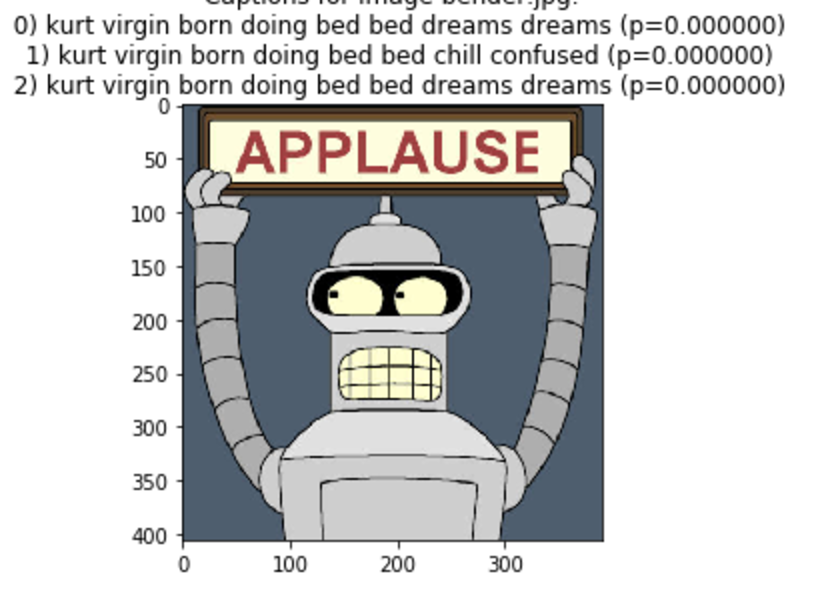
\includegraphics[width=\linewidth]{exp7-anec-2}
  %% \end{minipage}
  \caption{
    Resultados \emph{anecdóticos} del entrenamiento de la LSTM, a partir de una CNN superficial.
    Al igual que con la red \emph{Inception V3}, hay una considerable repetición de palabras.
    El desempeño mostrado sugiere pensar que la generalización de las imágenes pertenecientes
    al conjunto de datos no requiere de un modelo que explore, con gran detalle, sus características
    más intrínsecas.
    (Fuente: elaboración propia.)
  }
  \label{exp7:anec}
\end{table}

\begin{table}[h]
  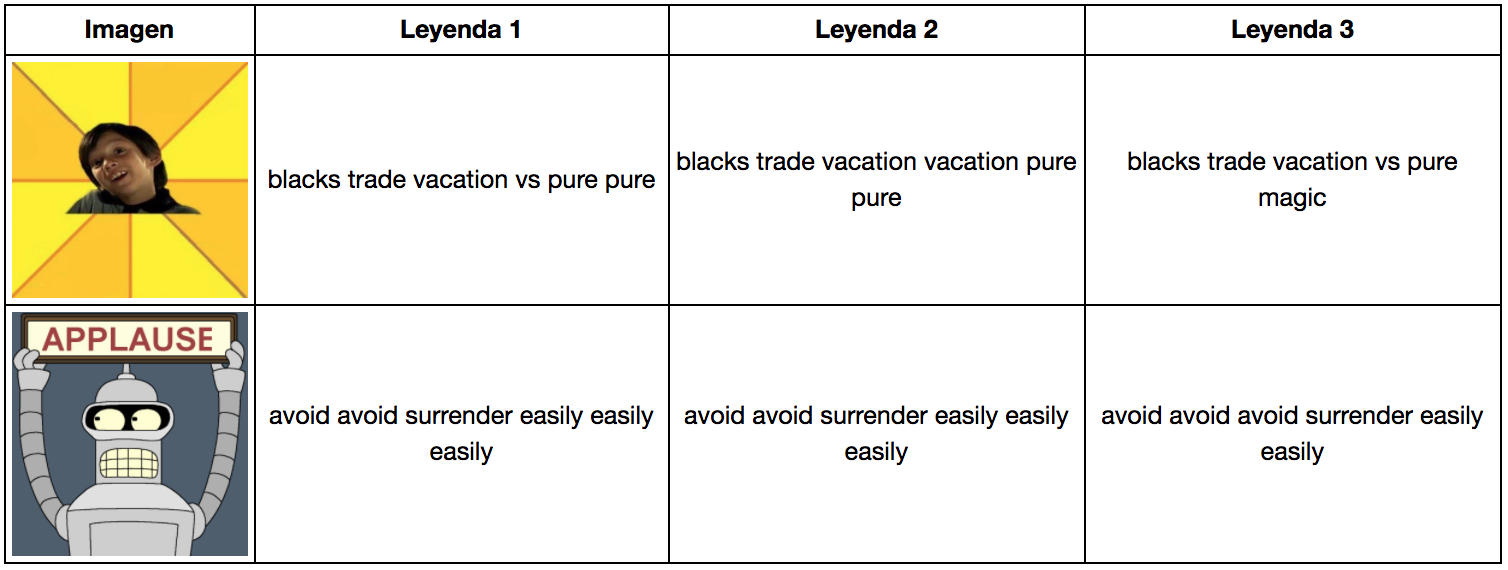
\includegraphics[width=\linewidth]{exp8-anec}
  %% \begin{minipage}[c]{\linewidth}
  %%   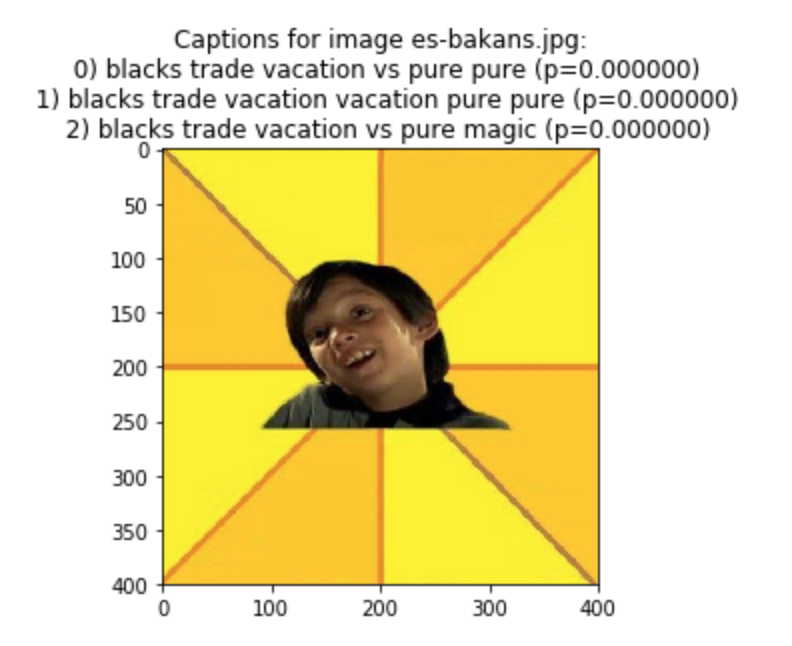
\includegraphics[width=\linewidth]{exp8-anec-1}
  %% \end{minipage}\hfill
  %% \begin{minipage}[c]{\linewidth}
  %%   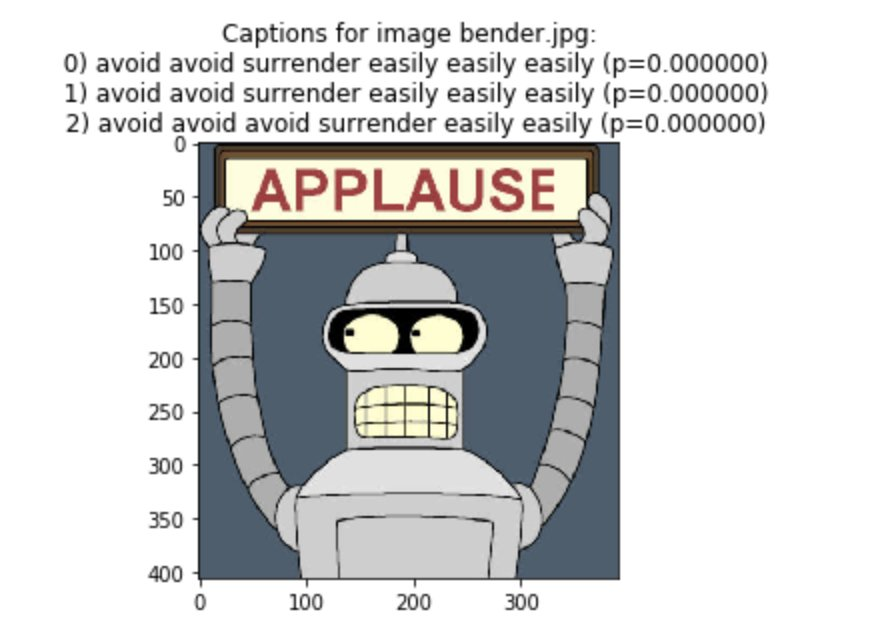
\includegraphics[width=\linewidth]{exp8-anec-2}
  %% \end{minipage}
  \caption[Nota al pie]{
    Resultados \emph{anecdóticos} del entrenamiento de la LSTM, a partir de una CNN superficial
    y 20 leyendas por personaje. Aquí cabe destacar que cuando una palabra sucede a otra, si éstas son distintas,
    la lógica entre \emph{categorías gramaticales} suele hacer sentido a juicio de un ser humano.
    Por ejemplo, la aparición de un artículo antes de un sustantivo o verbos a la mitad de la leyenda.
    (Fuente: elaboración propia.)
  }
  \label{exp8:anec}
\end{table}

%% \chapter{Figuras ilustrativas}

%% \newpage

%% \begin{table}[H]
%%   \centering
%%   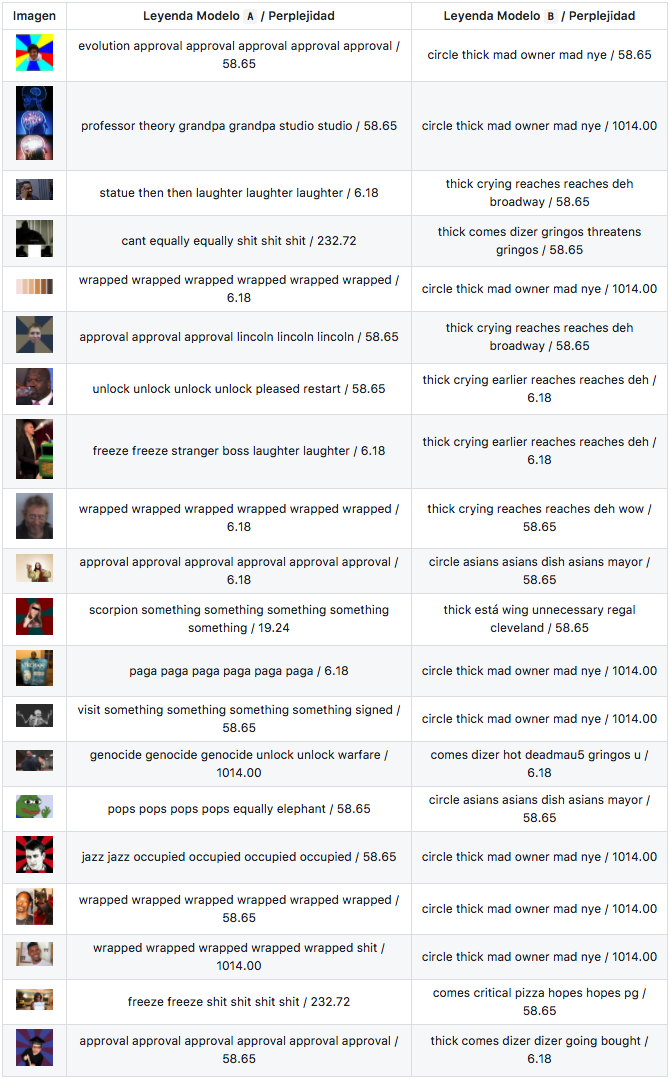
\includegraphics[width=\textwidth]{memesvsmemes}
%%   \caption{
%%     Dado un conjunto de memes nuevos, generamos leyendas para cada uno de éstos usando
%%     los dos mejores modelos obtenidos tras los experimentos de entrenamiento. Adicionalmente,
%%     para cada leyenda, calculamos la perplejidad contra el corpus obtenido de todas las leyendas\
%%     extraidas de internet.
%%   }
%%   \label{memesvsmemes}
%% \end{table}

%% \begin{table}[H]
%%   \centering
%%   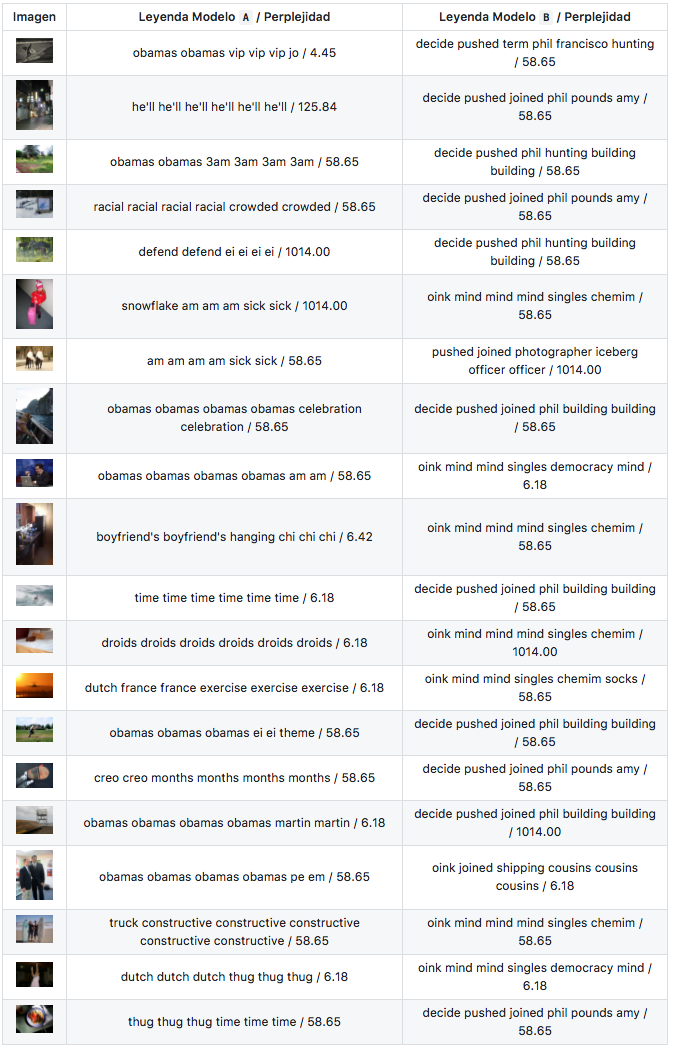
\includegraphics[width=\textwidth]{nonmemesvsmemes}
%%   \caption{
%%     Dado un conjunto de imágenes de \emph{ImageNet}, generamos leyendas para cada uno de éstos usando
%%     los dos mejores modelos obtenidos tras los experimentos de entrenamiento. Adicionalmente,
%%     para cada leyenda, calculamos la perplejidad contra el corpus obtenido de todas las leyendas\
%%     extraidas de internet.
%%   }
%%   \label{nonmemesvsmemes}
%% \end{table}
